\section{Map-based Skeletons}
\subsection{parMap}
\begin{center}
	\includegraphics[scale=0.7]{images/parMap}
\end{center}
\code{parMap} is probably the most common skeleton for parallel programs. We can implement it with \code{ArrowParallel} by repeating an arrow \code{arr a b} and then passing it into \code{parEvalN} to get an arrow \code{arr [a] [b]}. 
Just like \code{parEvalN}, \code{parMap} is 100 \% strict.
\begin{lstlisting}[frame=htrbl]
parMap :: (ArrowParallel arr a b conf, ArrowApply arr) =>
	conf -> (arr a b) -> (arr [a] [b])
parMap conf f =
	(arr $ \as -> (f, as)) >>>
	(first $ arr repeat >>>
		arr (parEvalN conf)) >>>
	app
\end{lstlisting}

\subsection{parMapStream}
\begin{center}
	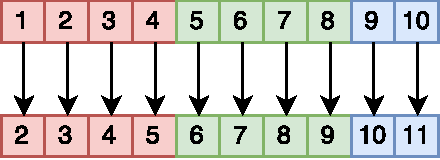
\includegraphics[scale=0.7]{images/parMapStream}
\end{center}
As \code{parMap} is 100\% strict it has the same restrictions as \code{parEvalN} compared to \code{parEvalNLazy}. So it makes sense to also have a \code{parMapStream} which behaves like \code{parMap}, but uses \code{parEvalNLazy} instead of \code{parEvalN}.
\begin{lstlisting}[frame=htrbl]
parMapStream :: (ArrowParallel arr a b conf, ArrowChoice arr, ArrowApply arr) =>
	conf -> ChunkSize -> arr a b -> arr [a] [b]
parMapStream conf chunkSize f =
	(arr $ \as -> (f, as)) >>>
	(first $ arr repeat >>>
		arr (parEvalNLazy conf chunkSize)) >>>
	app
\end{lstlisting}

\subsection{farm}
\begin{center}
	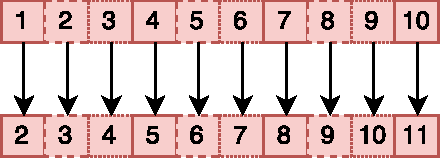
\includegraphics[scale=0.7]{images/farm}
\end{center}
\code{parMap} spawns every single computation in a new thread (at least for the instances of \code{ArrowParallel} we gave in this paper). This can be quite wasteful and a \code{farm} that equally distributes the workload over \code{numCores} workers (if numCores is greater than actualProcessorCount, the fastest processor(s) to finish will get more tasks) seems useful.
\begin{lstlisting}[frame=htrbl]
farm :: (ArrowParallel arr a b conf, ArrowParallel arr [a] [b] conf,
	ArrowChoice arr, ArrowApply arr) =>
	conf -> NumCores -> arr a b -> arr [a] [b]
farm conf numCores f =
	(arr $ \as -> (f, as)) >>>
	(first $ arr mapArr >>> arr repeat >>>
		arr (parEvalN conf)) >>>
	(second $ arr (unshuffle numCores)) >>>
	app >>>
	arr shuffle
\end{lstlisting}
The definition of \code{unshuffle} is
\begin{lstlisting}[frame=htrbl]
unshuffle :: Int
	-> [a]
	-> [[a]]
unshuffle n xs = [takeEach n (drop i xs) | i <- [0..n-1]]
\end{lstlisting}
, while \code{shuffle} is defined as:
\begin{lstlisting}[frame=htrbl]
shuffle :: [[a]]
	-> [a]
shuffle = concat . transpose
\end{lstlisting}
(These were taken from Eden's source code. \cite{eden_skel_shuffle})

\subsection{farmChunk}
\begin{center}
	\includegraphics[scale=0.7]{images/farmChunk}
\end{center}
As \code{farm} is basically just \code{parMap} with a different work distribution, it is, again, 100\% strict. So we define \code{farmChunk} which uses \code{parEvalNLazy} instead of \code{parEvalN} like this:
\begin{lstlisting}[frame=htrbl]
farmChunk :: (ArrowParallel arr a b conf, ArrowParallel arr [a] [b] conf,
	ArrowChoice arr, ArrowApply arr) =>
	conf -> ChunkSize -> NumCores -> arr a b -> arr [a] [b]
farmChunk conf chunkSize numCores f =
	(arr $ \as -> (f, as)) >>>
	(first $ arr mapArr >>> arr repeat >>>
		arr (parEvalNLazy conf chunkSize)) >>>
	(second $ arr (unshuffle numCores)) >>>
	app >>>
	arr shuffle
\end{lstlisting}

\subsection{parMapReduce}